\documentclass[a4]{article}

\usepackage[T1]{fontenc}
\usepackage[icelandic]{babel}
\usepackage{amsmath}
\usepackage{graphicx}
\usepackage{sidecap}
\usepackage[utf8]{inputenc}
\usepackage[left=1in,top=1in,right=1in,bottom=1in,nohead]{geometry}
\usepackage[framed,numbered,autolinebreaks,useliterate]{../mcode}
\usepackage{amsfonts}
\usepackage{epstopdf}

\lstset{language=MATLAB}
\title{Töluleg Greining\\ Heimaverkefni 3}
\date{\today{}}
\author{ 
  Bjarki Geir Benediktsson,\and
  Haukur Óskar Þorgeirsson,\and
  Matthías Páll Gissurarson \and
  Kennari: Máni Maríus Viðarsson
  }



\begin{document}
\begin{flushright}
  Bjarki Geir Benediktsson,\\
  Haukur Óskar Þorgeirsson,\\
  Matthías Páll Gissurarson\\
\end{flushright}

\begin{center}
 \textsc{ \LARGE Töluleg Greining\\
  Heimaverkefni 3\\
  \today{}
  }
  \end{center}
\vfill

\maketitle
\section{Forsagnar- og Leiðréttingaraðferð}
\subsection{}
\lstinputlisting[inputencoding=utf8]{adams_pc5.m}
\subsection{}
\lstinputlisting[inputencoding=utf8]{adams_pc5plot.m}
\lstinputlisting[inputencoding=utf8]{adams_pc5test.m}
Sjá myndir \ref{fig:adamspc5plot} og \ref{fig:adamspc5err}.
\begin{figure}[]
  \begin{center}
    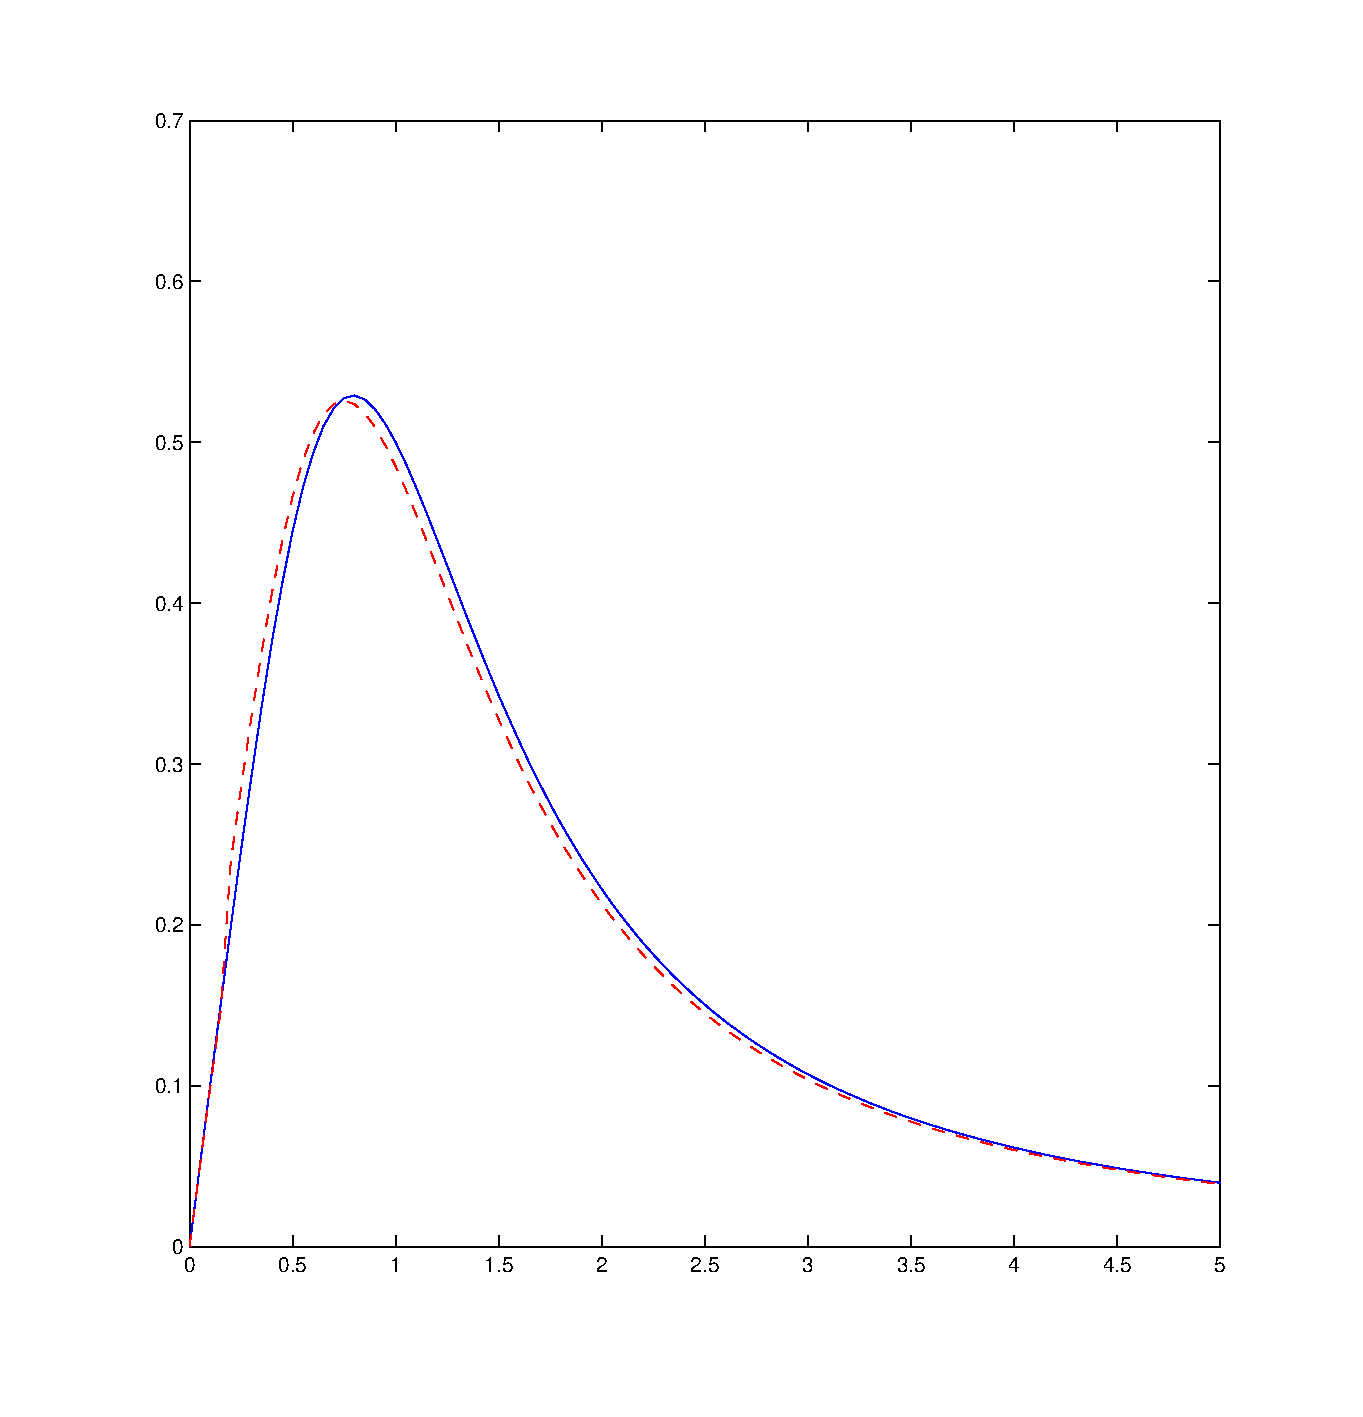
\includegraphics[scale=0.5]{adamspc5plot.eps}
  \end{center}
  \caption{Fallið sem prófa átti í 1, auk nálgun þess með adams\_pc5 sem rautt brotastrik}
  \label{fig:adamspc5plot}
\end{figure}
\begin{figure}[h]
  \begin{center}
    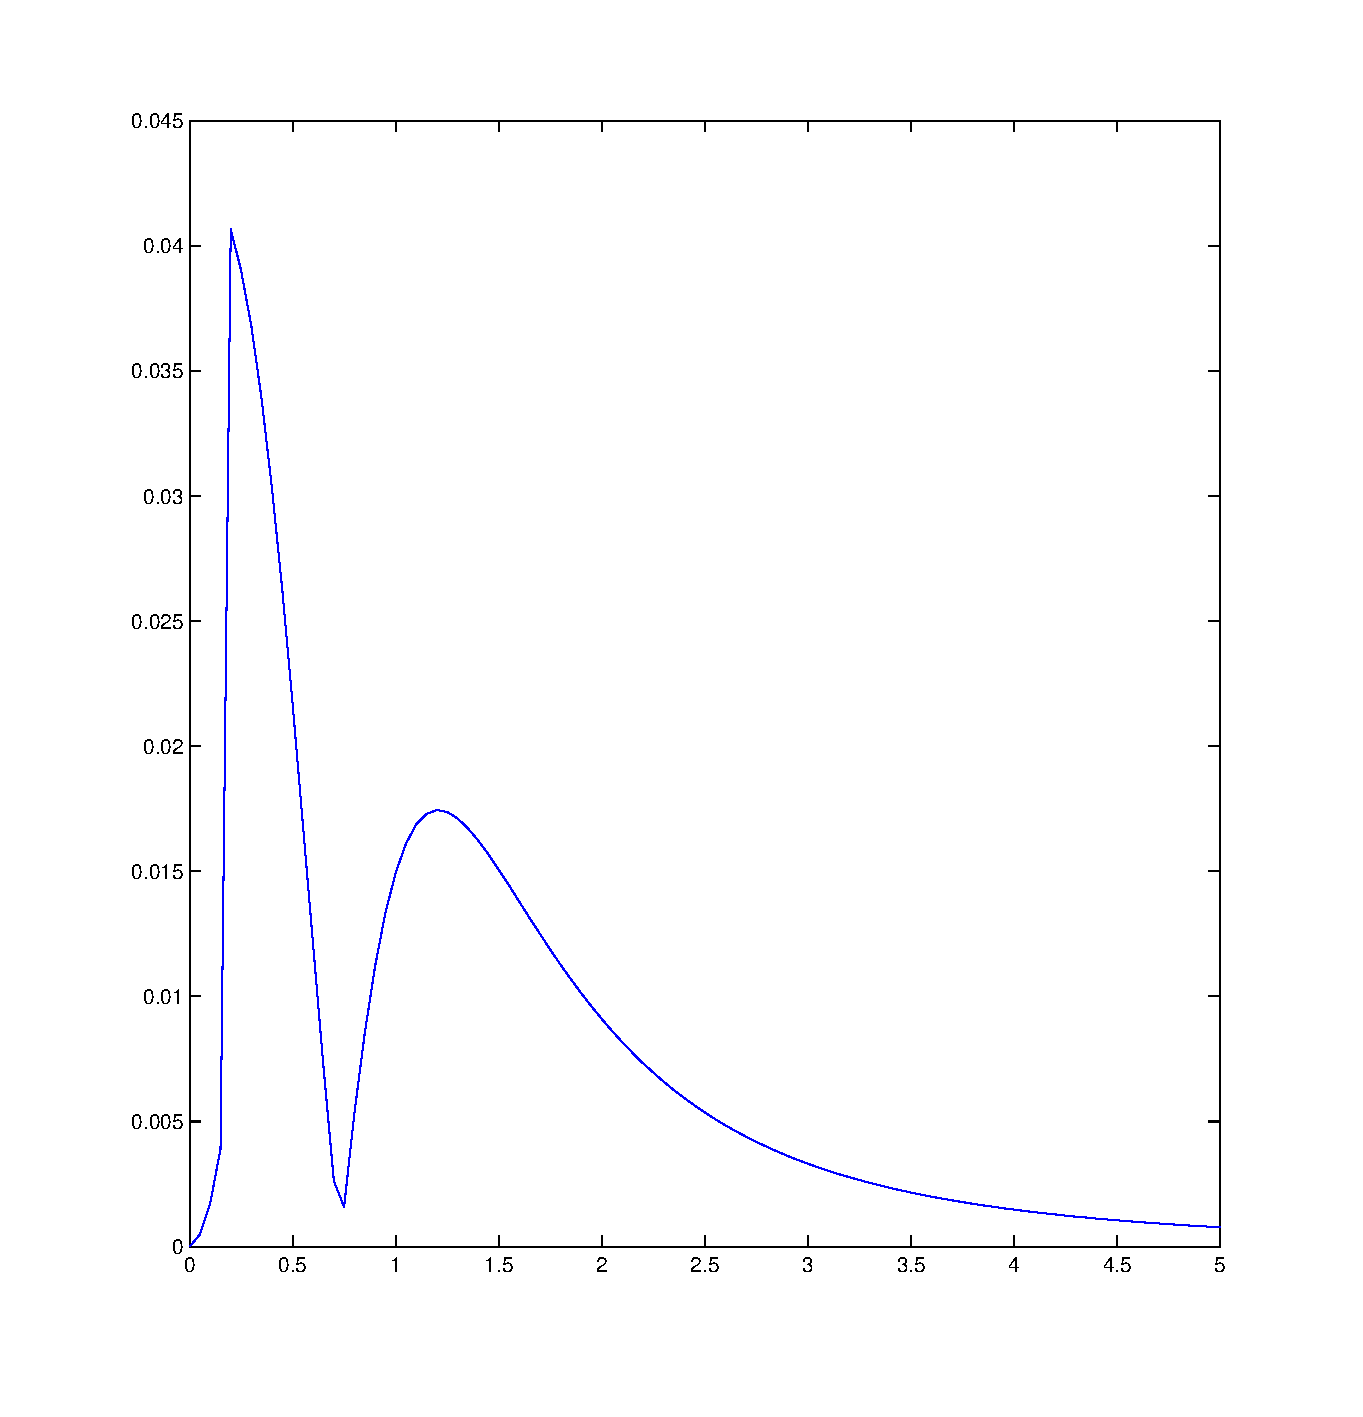
\includegraphics[scale=0.5]{adamspc5err.eps}
  \end{center}
  \caption{Skekkjan milli nálgunar þess með adams\_pc5 og fallsins sem prófa átti í 1 sem fall af t}
  \label{fig:adamspc5err}
\end{figure}
\subsection{}
til þess að fá heildarskekkju minni en $10^{-4}$ þurfti $h=\frac{1}{50000}=2*10^{-5}$

\subsection{Tímamælingar}
\lstinputlisting[inputencoding=utf8]{Timetake.m}
%athuga hvort það þurfi að breyta gildunum í take Taketime og uppfæra þá þessi gildi
Keyrsla á þessu forriti gaf eftirfarandi niðurstöður\\
\begin{tabular}{|c|c|}
\hline
fall		&meðatími \\\hline
adams\_pc5	&0,0082\\\hline
rkf45		&0,0024\\\hline
rkv56		&0,0027\\\hline
\end{tabular}


\section{Einfaldur pendúll}
Við fáum að þar sem $$\theta''(t) + \frac{g}{l} \cdot \sin{ \theta(t)} \Leftrightarrow \theta''(t) = -\frac{g}{l} \cdot \sin{\theta(t)}$$
  þá má rita $$\left\{ \begin{array}{l} y(t) = \theta'(t) \\ y'(t) = \theta''(t) = - \frac{g}{l} \cdot \sin{\theta(t)} \end{array} \right.$$
Notum þetta til að skilgreina eftirfarandi fall:
\lstinputlisting[inputencoding=utf8]{pendulODE.m}
\lstinputlisting[inputencoding=utf8]{pendulApprox.m}

Við notuðum síðan þetta til að teikna hreyfimyndir, en það var gert með
\lstinputlisting[inputencoding=utf8]{pendull.m}

Með því að prófa nokkur gildi og horfa á útkomuna, þá komumst við að því að upphafhornið
$\theta_0 = 0.42$ gaf okkur frekar góða nálgun að 3 umferð, en eftir það fóru lausnirnar að greinast í sundur.

Til þess að svo gera hreyfimyndina þar sem útslagið er stórt var notaður eftirfarandi forritsbútur:
\lstinputlisting[inputencoding=utf8]{hr2.m}

\section{Róla}
  Við athugum að jafnan er eins og í 2, nema nú er lengdin auk þess fall af t. því fæst jöfnuhneppið
  $$\left\{ \begin{array}{l} y(t) = \theta'(t) \\ y'(t) = \theta''(t) = - \frac{g}{s(t)} \cdot \sin{\theta(t)} \end{array} \right.$$ 
  en $$s(t) = l + a*(cos \omega t + \varphi),$$
  þar sem l er lengdin, a er ústlagið, $\omega$ er horntíðnin og $\varphi$ er fasahliðrunin.
  
  Eftirfarandi tvö föll voru gerð til þess að nota með adams\_pc5, en fyrra er fyrir rólu sem er að hægja á sér og seinna er fyrir rólu sem er að hámarka útslagið. Munurinn liggur í mismunandi fasahliðrunum.
  \lstinputlisting[inputencoding=utf8]{roluODEmin.m}
  \lstinputlisting[inputencoding=utf8]{roluODEmax.m}

  Til þess svo að teikna meðfylgjandi myndbönd var notast við eftirfarandi skrá og pendull.m úr fyrri lið.
  \lstinputlisting[inputencoding=utf8]{hr3.m}.
  
  Útslagið örvaðist mest þegar $\omega = 1/T$ eins og gefið var í 3
 örvunin var jákvæð (sveiflan jókst) þegar  fasahornið var $\pi$ í byrjun en neikvæð ef fasahornið var  $\varphi = 0$, þá hægði maður á rólunni.
 Munurinn liggur í hvenær maður styttir og lengir bandið, en ef fasahornið er $\pi$%er nokkuð viss um að þetta sé rétt svona
, þá er mesta lengingin í miðjunni og minnst í endapunktunum,
  en öfugt er farið þegar hægt er á rólunni. \\
Orsökina fyrir þessari hegðun í okkar einfalda módeli er að finna í orkubúskap kerfisins en við gerum ráð fyrir að enginn orka fari í að hreyfa massamiðjuna upp og niður róluna\\
þegar rólan er í hæstu stöðu þá er öll orka kerfisins stöðuorka og því ofar sem massamiðjan er þeim mun meiri er orka kerfisins og á svo lengi sem sveiflan er ekki meiri en $\frac{\pi}{2}$ frá lóðréttu þá færir það massamiðjuna ofar að stytta róluna\\
eins þegar rólan er lárétt (í mijunni) þá er öll orka kerfisins skriðorka og því neðar sem massamiðjan er því meiri stöðuorka hefur verið losuð í skriðorku og augljóslega er massamiðjan neðar þegar lengt er í rólunni í þessari stöðu\\
þegar fasahorninu er breytt þannig að rólan sé styðst í lóðréttu stöðunni og lengst í mesta útslaginu þá er ekki öll orkan í kerfinu færð milli skriðorku og stöðuorku í hverri sveiflu og því glatast orka úr kerfinu \\ Rétt er að athuga að þetta brýtur ekki gegn orkuvarðveislulögmálinu af því að sú orka sem hverfur (eða verður til þegar verið var að auka sveifluna) fer í vinnuna að færa massamiðjuna upp og niður róluna\\
einnig sést í forritinu fyrir jákvæða örvun að þegar útslagið er orðið meira en $\frac{\pi}{2}$ þá er næsta sveifla á eftir ekki hærri þetta er vegna þess að þegar sveiflan er orðin þetta stór þá færist massamiðjan neðar við það að stytt sé í rólunni og því er minni stöðuorka til staðar til þess að breyta í skriðorku fyrir næstu sveiflu. (þessar upplýsingar hefðu verið vel þegnar fyrir um 15 árum síðan þegar undirritaður var að reyna að ná heilum hring í rólunum á leikvellinum)

\section{Kúlupendúll}
 Jöfnuhneppið er einfaldlega það sama og gefið er í liðnum, en það má sjá í 
\lstinputlisting[inputencoding=utf8]{kulupendulODE.m}

 Eftirfarandi forritsbútur var notaður til að búa til myndbandið.
\lstinputlisting[inputencoding=utf8]{hr4.m}
 Það var gert með hjálp eftirfarandi falls, sem er pendúlsteiknifallið breytt til þess að ráða við þrívídd.
\lstinputlisting[inputencoding=utf8]{pendull3d.m}

\section{Lorenz Attractor}
Við ákváðum að gera myndaband af Lorentz Attractorum, en það eru lausnir á diffurjöfnum sem gefa ákaflega fallega ferla.
Diffurjöfnuna má finna hér, en við henni var bættur möguleiki til að taka inn fasta sem notaðir eru, en það er til þess
að auðvelda okkur að teikna margar eindir í einu.

\lstinputlisting[inputencoding=utf8]{lorenzODE.m}

Eftirfarandi forrit var svo búið til til þess að gera myndbandið, en það tekur sem viðföng fastana og upphafsstaðsetningar
eindanna, svo auðvelt væri að bæta við fleirum.
\lstinputlisting[inputencoding=utf8]{lorenzAnim.m}

Eftirfarandi forritsbútur var svo gerður sem býr til myndbandið sem skilað var inn.
\lstinputlisting[inputencoding=utf8]{hr5.m}

\vspace{20 mm}
Að skýrsluni unnu :
\hspace{0.5cm} \makebox[1.5in]{\hrulefill}
\hspace{0.5cm} \makebox[1.5in]{\hrulefill}
\hspace{0.5cm} \makebox[1.5in]{\hrulefill}
\end{document}
